\begin{exercise}
\begin{figure}[H]
\centering
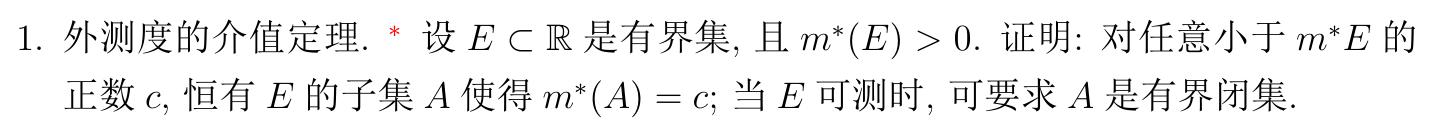
\includegraphics[width=\textwidth]{2-hw7-2025042112.png}
% \caption{}
\label{}
\end{figure}
\end{exercise}
\begin{proof}
$E\subset[a,b]$ for some $a, b\in \mathbb{R}$, let
\[
f(x)\coloneqq m^{*}(E\cap[a,x))\qquad x\in(a,b]
\]
For $\Delta x>0$, we have
\[
f(x+\Delta x)-f(x)=m^{*}(E\cap[x,x+\Delta x))\leq m^{*}[x,x+\Delta x)=\Delta x
\]
\[
f(x)-f(x-\Delta x)=m^{*}(E\cap[x-\Delta x,x))\leq \Delta x
\]
Thus $f\in C(a,b]$. We have $f(a+)=0,f(b)=m^*E$. Applying the intermediate value theorem to $f$, for any $c\in (0,m^{*}E]$, there exists $x\in(a,b]$ s.t. $f(x)=c$, i.e.  $m^{*}(E\cap[a,x))=c$. Let $A=E\cap[a,x)$ then we are done.
\end{proof}

\begin{exercise}
\begin{figure}[H]
\centering
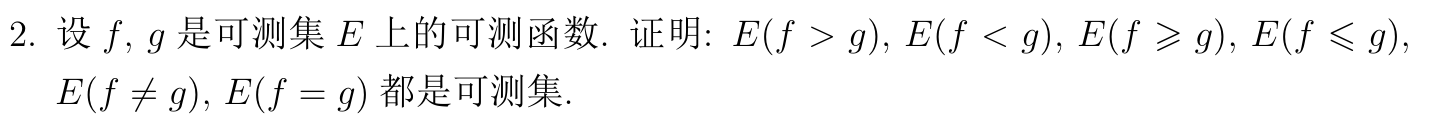
\includegraphics[width=\textwidth]{4-hw7-2025042112.png}
% \caption{}
\label{}
\end{figure}
\end{exercise}
\begin{proof}
Since $f$ and $g$ are measurable functions over $E$, we have $E (f>c)\in \mathcal{M}, E (g>c)\in \mathcal{M}$ for any $c\in \mathbb{R}$. Then
\[
E(f>g)=\bigcup_{r\in \mathbb{Q}}(E(f>r)\cap E(g\leq r))=\bigcup_{r\in \mathbb{Q}}(E(f>r)\cap E(g>r)^{c})\in \mathcal{M}
\]
Similarly,
\[
E(g>f)\in \mathcal{M}
\]
Then
\[
E(f\geq g)=E(f<g)^{c}\in \mathcal{M},\quad E(f\leq g)=E(f>g)^{c}\in \mathcal{M}
\]
\[
E(f\neq g)=E(f>g)\cup E(f<g)\in \mathcal{M}
\]
\[
E(f=g)=E(f\leq g)\cap E(f\geq g)\in \mathcal{M}
\]
\end{proof}

\begin{exercise}
\begin{figure}[H]
\centering
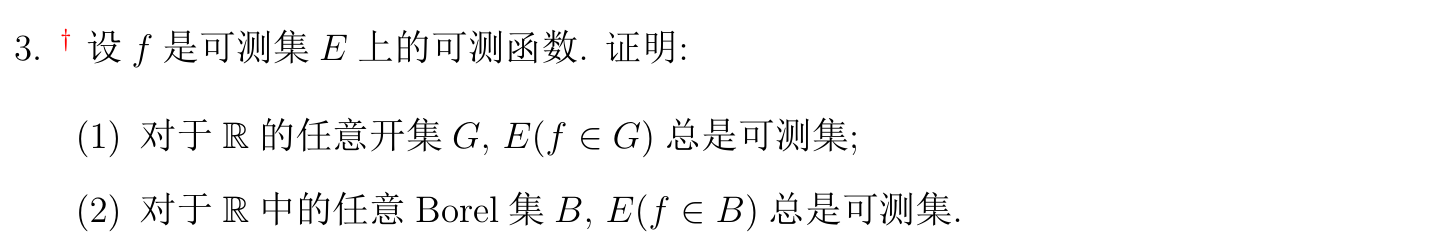
\includegraphics[width=\textwidth]{5-hw7-2025042112.png}
% \caption{}
\label{}
\end{figure}
\end{exercise}
\begin{proof}
(1) Since $G$ is open in $\mathbb{R}$, we have disjoint $\{ (a_n,b_n) \}_{n=1}^{\infty }$ s.t.
\[
E(f\in G)=E\left( f\in\bigsqcup_{n=1}^{\infty}(a_n,b_n) \right)=\bigcup_{n=1}^{\infty} (E(f>a_n)\cap E(f<b_n))\in \mathcal{M}
\]
(2) For $A,B$ open or closed in $\mathbb{R}$, we have
\[
E(f\in A)\in \mathcal{M}, E(f\in B)\in \mathcal{M}
\]
Then
\[
E(f\in A\cap B)=E(f\in A)\cap E(f\in B)\in \mathcal{M}
\]
\[
E(f\in A\cup B)=E(f\in A)\cup E(f\in B)\in \mathcal{M}
\]
\[
E(f\in A^{c})=E(f\in A)^{c}\in M
\]
Therefore for any Borel set $B$,
\[
E(f\in B)\in \mathcal{M}
\]
\end{proof}

\begin{exercise}
\begin{figure}[H]
\centering
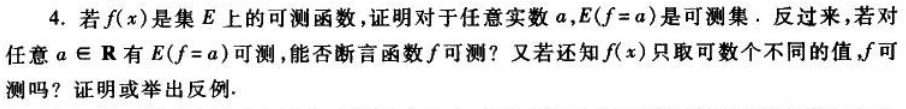
\includegraphics[width=\textwidth]{6-hw7-2025042112.png}
% \caption{}
\label{}
\end{figure}
\end{exercise}
\begin{proof}
$E (f=a)=E (f\geq a)\cap E (f\leq a)\in \mathcal{M}$.
\begin{figure}[H]
\centering
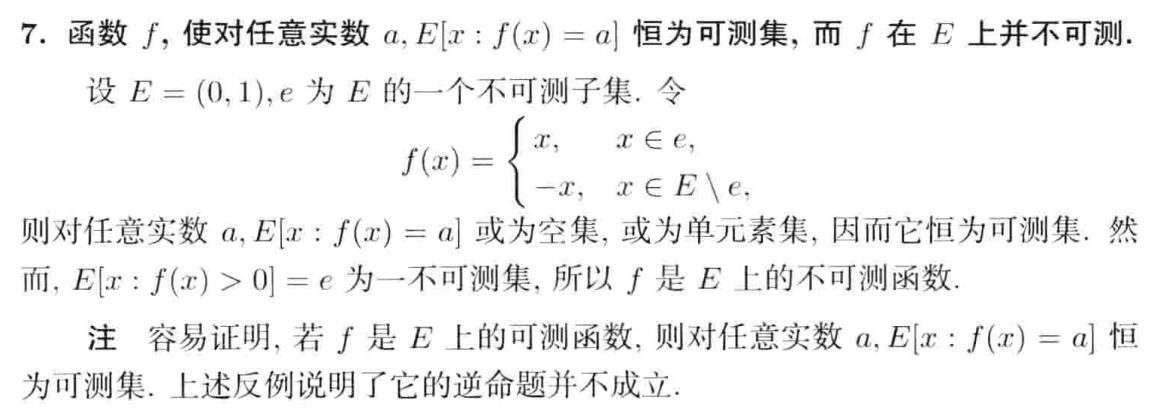
\includegraphics[width=\textwidth]{15-hw7-2025042112.png}
% \caption{}
\label{}
\end{figure}
If $\{ f(x):x\in E \}$ is countable, then for any $c\in E$, $E(f>c)$ is countable, thus measurable. Hence $f$ is measurable.
\end{proof}

\begin{exercise}
\begin{figure}[H]
\centering
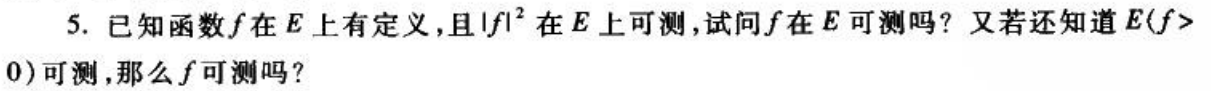
\includegraphics[width=\textwidth]{7-hw7-2025042112.png}
% \caption{}
\label{}
\end{figure}
\end{exercise}
\begin{proof}
\begin{figure}[H]
\centering
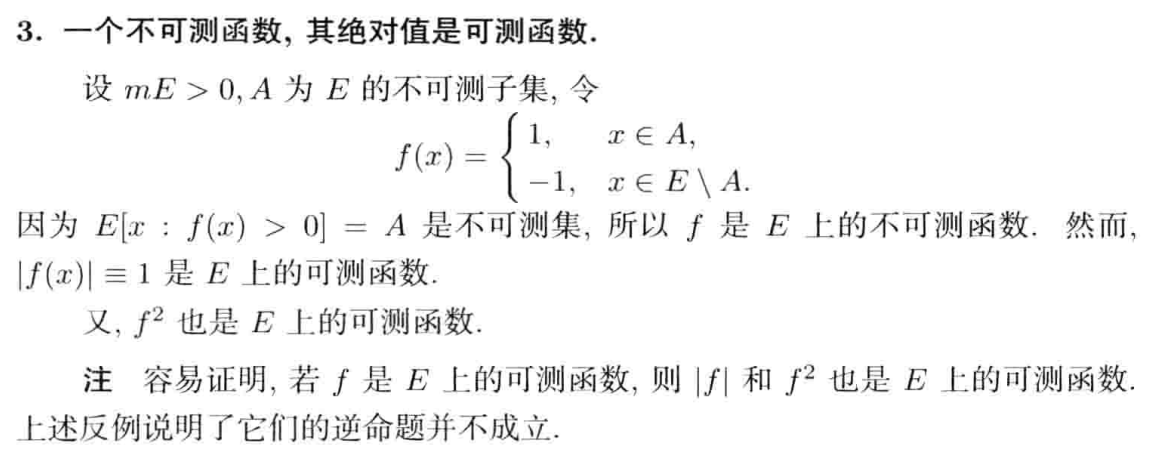
\includegraphics[width=\textwidth]{16-hw7-2025042112.png}
% \caption{}
\label{}
\end{figure}
Since $\lvert f \rvert ^2$ is measurable, then $E (f=0)=E (\lvert f \rvert ^2=0)\in \mathcal{M}$. For $c>0$, $E (\lvert f \rvert ^2>c^2)=E (f>c)\cup E (f<-c)\in \mathcal{M}$. Since $E (f>0)\in \mathcal{M}$, then
\[
E(f>c)=E(\lvert f \rvert ^2>c^2)\cap E(f>0)\in \mathcal{M}
\]
\[
E(f\geq -c)=E(f<-c)^{c}=(E(\lvert f \rvert ^2>c^2)\cap E(f>0)^{c})^{c}\in \mathcal{M}
\]
Then
\[
E(f>-c)=\bigcap_{n=1}^{\infty} E\left( f\geq -c-\frac{1}{n} \right)\in \mathcal{M}
\]
Therefore for any $c\in \mathbb{R}$, we have
\[
E(f>c)\in \mathcal{M}
\]
Hence $f$ is measurable.
\end{proof}

\begin{exercise}
\begin{figure}[H]
\centering
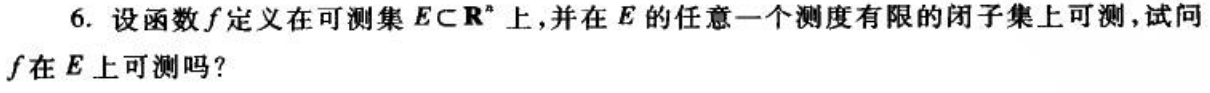
\includegraphics[width=\textwidth]{8-hw7-2025042112.png}
% \caption{}
\label{}
\end{figure}
\end{exercise}
\begin{proof}
There is a $F_{\sigma}$ set $F$ contained in $E$ for which $m^{*}(E\setminus F)=0$. $f$ is measurable on $F$ (it's trivial). For any $c\in \mathbb{R}$,
\[
m^{*}((E\setminus F)[f>c])\leq m^{*}(E\setminus F)=0 
\]
Thus $(E\setminus F)[f>c]\in \mathcal{M}$,
\[
E[f>c]=F[f>c]\cup(E\setminus F)[f>c]\in\mathcal{M}
\]
\end{proof}

\begin{exercise}
\begin{figure}[H]
\centering
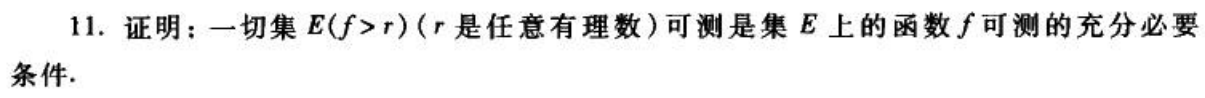
\includegraphics[width=\textwidth]{9-hw7-2025042112.png}
% \caption{}
\label{}
\end{figure}
\end{exercise}
\begin{proof}
Suppose that $f$ is measureable, then $E (f>r)\in \mathcal{M}$ for any $r\in \mathbb{Q}$. Conversely, $E (f>r)\in \mathcal{M}$ for any $r\in \mathbb{Q}$ then for any $c\in \mathbb{R}$, there is a rational sequence $\{ r_n \}_{n=1}^{\infty}\to c$ with $r_n>c$. Then
\[
E(f>c)=\bigcap_{n=1}^{\infty} E(f>r_n)\in \mathcal{M}
\]
Therefore $f$ is measurable on $E$.
\end{proof}

\begin{exercise}
\begin{figure}[H]
\centering

\includegraphics[width=\textwidth]{10-hw7-2025042112.png}
% \caption{}
\label{}
\end{figure}
\end{exercise}
\begin{proof}
当指标集 $I$ 为不可数集,$\{ f_{\alpha} \}_{\alpha\in I}$ 的上确界函数 $\sup_{\alpha}f_{\alpha}$ 不一定可测,反例可取 $W\subset[0,1]$ 为不可数集,对 $\alpha\in W$,作函数
\[
f_{\alpha}(x)=\begin{cases}
1 & x=\alpha \\
0 & x\neq \alpha
\end{cases}\qquad x\in[0,1]
\]
则 $S(x)=\chi_{W}(x)$ 并不可测.

如果加上了 $f_{\alpha}$ 连续的条件,那么对于任意的 $c\in \mathbb{R}$,
\[
\begin{aligned}
E[\sup_{\alpha}f_{\alpha}\geq c] & =\bigcap_{j=1}^{\infty} \bigcup_{\alpha\in I}\left\{  x\in E:f_\alpha(x)> c-\frac{1}{j}  \right\} \\
 & =\bigcap_{j=1}^{\infty} \bigcup_{\alpha\in I}f_{\alpha}^{-1}\left( c-\frac{1}{j},\infty \right)
\end{aligned}
\]
由于 $f_{\alpha}\in C(E)$,故 $f^{-1}_{\alpha}\left( c-\frac{1}{j},\infty \right)$ 是开集,开集的任意并也是开集,故 $\bigcup_{\alpha\in I}f^{-1}_{\alpha}\left( c-\frac{1}{j},\infty \right)$ 是开集,于是 $E[\sup_{\alpha}f_{\alpha}\geq c]$ 是 $G_{\delta}$ 集,故可测. 于是 $f$ 可测.
\end{proof}

\begin{exercise}
\begin{figure}[H]
\centering
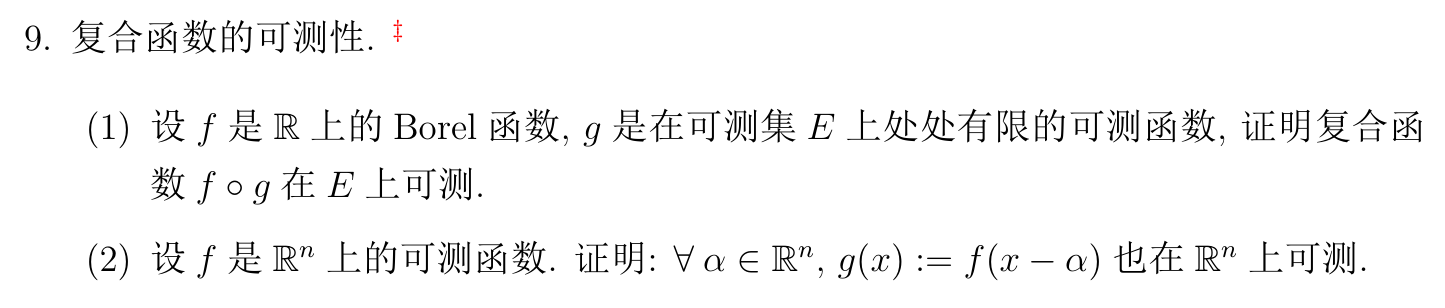
\includegraphics[width=\textwidth]{11-hw7-2025042112.png}
% \caption{}
\label{}
\end{figure}
\end{exercise}
\begin{proof}
(1)

\begin{remark}
\begin{figure}[H]
\centering
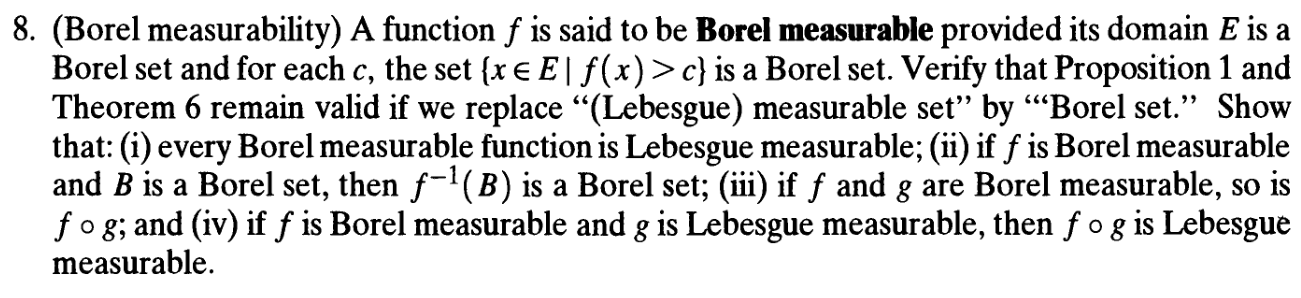
\includegraphics[width=\textwidth]{1-hw7-2025042211.png}
% \caption{}
\label{}
\end{figure}
\end{remark}
\href{https://www.bilibili.com/video/BV1Wq4y1P7d3?spm_id_from=333.788.videopod.episodes&vd_source=b55594d2ba73cdd7666e94ca2cf2fe93&p=8}{3.8\_哔哩哔哩\_bilibili}

\begin{lemma}
If $g$ is Lebesgue measurable, and $B$ is a Borel set, then $g^{-1}(B)\in \mathcal{M}$.\label{1d07c0}
\end{lemma}

\begin{proof}
For any open interval $I$, we have $g^{-1}(I)\in \mathcal{M}$. Given $\mathcal{O}\subset \mathbb{R}$, open, then $\mathcal{O}=\bigcup_{n=1}^{\infty}I_n$. In open interval
\[
f^{-1}(\mathcal{O})=\bigcup_{n=1}^{\infty} f^{-1}(I_n)\in \mathcal{M}
\]
Let $\mathcal{A}\coloneqq \{ A\subseteq \mathbb{R}:f^{-1}(A)\in \mathcal{M} \}$. Every open set in $\mathbb{R}$ is contained in $\mathcal{A}$. In particular, $\mathbb{R}\in \mathcal{A}$. $\mathcal{A}$ is closed under completion and coutable union. (left as an exercise) Hence the conclusion follows.
\end{proof}
To prove that $f\circ g$ is Lebesgue measurable function, it suffices to check that $(f\circ g)^{-1}(\mathcal{O})\in \mathcal{M}$ for any open set $\mathcal{O}\subset \mathbb{R}$. Note that
\[
(f\circ g)^{-1}(\mathcal{O})=g^{-1}(f^{-1}(\mathcal{O}))
\]
Since $f$ is Borel function and $\mathcal{O}$ is Borel set, $f^{-1}(\mathcal{O})\in \mathcal{B}$. By \cref{1d07c0}, $g^{-1}(f^{-1}(\mathcal{O}))\in \mathcal{M}$, which yields the conclusion.

(2) For any open set $\mathcal{O}\subset \mathbb{R}^{n}$,
\[
\begin{aligned}
g^{-1}(\mathcal{O}) & =\{ x\in \mathbb{R}^{n}:g(x)\in \mathcal{O} \} \\
 & =\{ x\in \mathbb{R}^{n}:f(x-\alpha)\in \mathcal{O} \} \\
 & =\{ x+\alpha\in \mathbb{R}^{n}:f(x)\in \mathcal{O} \} \\
 & =\underbrace{ f^{-1}(\mathcal{O}) }_{ \in \mathcal{M} }+\alpha \in \mathcal{M}
\end{aligned}
\]
Hence the conclusion follows.
\end{proof}

\begin{exercise}
\begin{figure}[H]
\centering
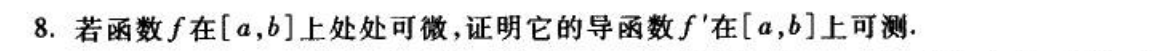
\includegraphics[width=\textwidth]{12-hw7-2025042112.png}
% \caption{}
\label{}
\end{figure}
\end{exercise}
\begin{proof}
Let
\[
f_n(x)\coloneqq \frac{f\left( x+\frac{1}{n} \right)-f(x)}{\frac{1}{n}}\qquad x\in[a,b)
\]
Then
\[
f'(x)=\lim_{ n \to \infty } f_n(x)
\]
Since $f\in \mathcal{D}[a,b]\subset \mathcal{C}[a,b]$, $f$ is measurable on $[a,b]$. Thus $f_n$ is measurable.

For any  $c\in \mathbb{R}$,
\[
\begin{aligned}
\{ x\in[a,b):f'(x)>c \} & =\{ x\in[a,b):\lim_{ n \to \infty } f_n(x)>c \} \\
 & =\bigcap_{n=1}^{\infty} \bigcup_{n=k}^{\infty}\underbrace{ \{ x\in[a,b):f_n(x)>c \}  }_{ \in \mathcal{M} } \in \mathcal{M }
\end{aligned}
\]
\begin{lemma}
设 $E\subset \mathbb{R}^{n}$,若存在 $\mathbb{R}^{n}$ 中可测集 $A$, 使得 $m^{*}(E\Delta A)=0$,则 $E\in \mathcal{M}$, 且有 $m(A)=m(E)$.\label{0feb41}
\end{lemma}

\begin{proof}
Trivial.
\end{proof}
Put $A=\{ x\in[a,b):f'(x)>c \}$ and $E=\{ x\in[a,b]:f'(x)>c \}$, then
\[
m^{*}(E\Delta A)\leq m^{*}(\{ b \})=0
\]
By \cref{0feb41}, we have $E\in \mathcal{M}$. Hence the conclusion follows.

\end{proof}

\begin{exercise}
\begin{figure}[H]
\centering
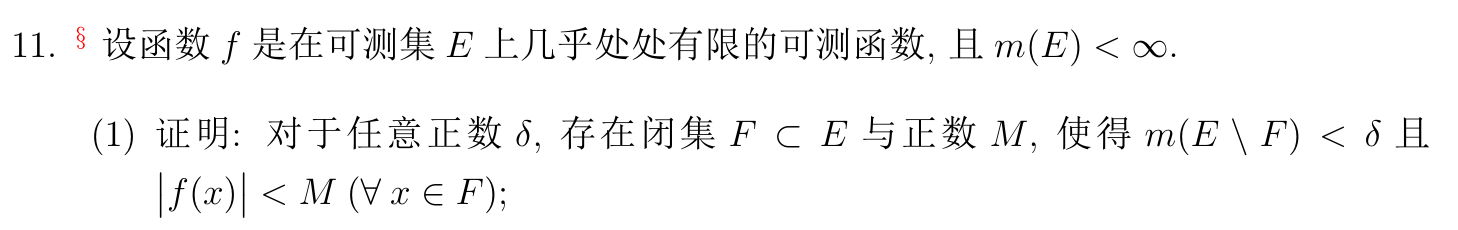
\includegraphics[width=\textwidth]{13-hw7-2025042112.png}
% \caption{}
\label{}
\end{figure}
\begin{figure}[H]
\centering
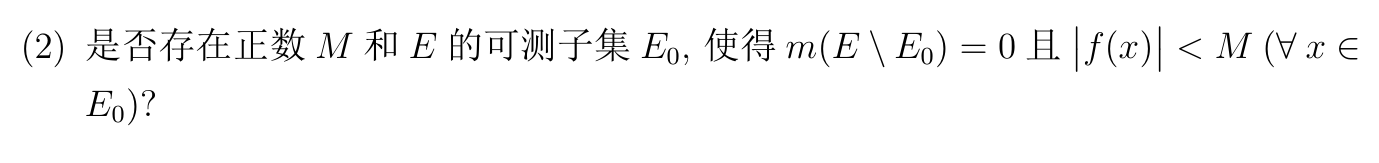
\includegraphics[width=\textwidth]{14-hw7-2025042112.png}
% \caption{}
\label{}
\end{figure}
\end{exercise}
\begin{proof}
(1)
\[
0=E[f=\infty]=\bigcap_{n=1}^{\infty} E[\lvert f \rvert > n]=\lim_{ n \to \infty } E[\lvert f \rvert > n]
\]
That is, for any $\delta>0$, there exists $n>0$ s.t.
\[
m(E[\lvert f \rvert > n])<\delta
\]
Let $F\coloneqq E[\lvert f \rvert\leq n]\subset E$ and $M=n+1$, then $m(E\setminus F)=m(E[\lvert f \rvert>n])<\delta$, and $\lvert f(x) \rvert\leq n<M$.

(2) No. Consider $E=[0,1]$ and
\[
f_n(x)=\sum_{n=1}^{\infty} \chi_{\left[ 0,\frac{1}{n} \right]}(x)
\]
If $\lvert f (x) \rvert<M,\forall x\in E_0$, then $E_0\subset(M^{-1},1]$. Thus $E\setminus E_0\supset[0,M^{-1}]$, $m(E\setminus E_0)\geq m[0,M^{-1}]=M^{-1}>0$.
\end{proof}
